\documentclass[11pt]{report}
\usepackage{standalone}
\graphicspath{ {images/} }
\setcounter{tocdepth}{5}
\setcounter{secnumdepth}{5}
\usepackage{natbib}
\bibliographystyle{agsm}
\usepackage{etoolbox}
\setlength{\parindent}{0em}
\setlength{\parskip}{0.25em}
\usepackage[raggedright]{titlesec}
\usepackage{hyperref}
\usepackage{capt-of}
\patchcmd{\bibliography}{\section*}{\section}{}{}
\titlespacing*{\chapter}{0pt}{-40pt}{10pt}
\titleformat{\chapter}[block]{\normalfont\huge\bfseries}{\thechapter}{15pt}{}
\usepackage{rotating}
\usepackage[titletoc]{appendix}
\usepackage{pgfgantt}
\usepackage{graphicx, rotating, caption, lscape, threeparttable}% \usepackage{amsmath}
\usepackage{array}
\usepackage{pdflscape}
\usepackage{geometry}
\usepackage{listings}
\usepackage[T1]{fontenc}
\usepackage[norsk,nameinlink]{cleveref}
\usepackage{multirow}



\begin{document}
\chapter{Experiments and Testing}

The designed and implemented system was practically applied to the semantic classification of the tweets regarding the discussion of  ``Britain Leaving the European Union''.
\\

\section{Tweet Collection Experiment}
Previous system's as stated in the related work used a set group of seed hashtags for which they collected tweets for and used as distant labels in their classification models. Instead of manually choosing the seed hashtags like previous Systems the experimentation choice was taken to extrapolate a seed hashtag set to use for collection and distant labelling. Initially, tweets containing either \#Brexit, \#VoteLeave and \#VoteRemain were collected. After collecting tweets from the day of referendum (23/06/2016) up until the initiation of the Brexit negotiations (18/06/2017), the Jacquard's Distance Function (see Figure \ref{fig:distance}) was applied on each of the hashtags found within the tweets to compare the similarity of each of the tweets containing the hashtags discovered and the tweets containing seed hashtags. The result was \textbf{similar\textunderscore hashtags.csv}; an ordered matrix of discovered hashtags that were similar to one or more of the seed hashtags. From the resulting similar  matrix, a bigger seed hashtag set was chosen (see Figure \ref{fig:seed}) whilst manually ignoring anomalous hashtags which were outliers and not on the discussion topic. 

\begin{center}
\[\forall x. \:\: \forall y. \:\: d_J(x, y)=1 - J(x,y) = 1 - \frac{|x \cap y|}{|x \cup y|}\ = 1 - \frac{|x \cap y|}{|x| + |y| - |x \cap y|}\]
\[where\:x = Set(tweets\:containing\:a\:unique\:discovered\:hashtag),\] 
\[y = Set(tweets\:containing\:a\:seed\:hashtag)\] 
\[and\:d_J(x, y) = Jacquard\:Distance\:Function\]
\captionof{figure}{Jacquard Distance Formula Function.}
\label{fig:distance}
\end{center}
\vspace{0.5cm}

\begin{center}
\#BREXIT \#ARTICLE50 \#BREXITDEBATE
                    \#BREXITMEANSBREXIT \#EUREFERENDUM \#EUREF
                    \#VOTELEAVE \#BREXITEER \#IVOTEDLEAVE \#LEAVEEU
                  \#TAKEBACKCONTROL \#VOTEOUT
				\#STRONGERIN \#REMAIN \#REMOANER \#REMAININEU
                  \#VOTEREMAIN \#STRONGERTOGETHER
\captionof{figure}{Generated Seed Hashtag Set.}
\label{fig:seed}
\end{center}
\clearpage

\section{Testing Methodologies}
The goal of testing within the System was to develop an effective test suite to verify and automate the testing of System behaviour. Tests were written for new functionality as the System functionality was developed, and thus the test methodology of Regression Testing was employed to ` provide a certain confidence that no new errors are introduced into previously tested code' \citep{MucciniSoftwarearchitecturebasedregression2006} when new changes to the system were implemented. The act of regression testing consists of running the entire suite of tests against new versions of the System to ensure expected System behaviour is upheld and was achieved through running of the test suite manual during local development of the System and automatically during the deployment of the System via a test step within the deployment pipeline (see Continuous Integration).

\section{Testing Strategy}
The System was tested using a mix of functional and non-functional testing, the types of testing carried out and the area for which they test is summarized in table /ref

\begin{center}
\begin{tabular}{ |p{3.5cm}||p{3.5cm}|p{7cm}|}
\hline
 Func. / Non-Func. & Testing Type & Scope of Test \\
 \hline
 Functional & Unit & Python Modules of Code\\
 \hline
 Functional & Integration & Interaction between Python Modules\\
 \hline
Functional & Validation & Correctness of Designed Classification Models\\
 \hline
Non-Functional & Load & Impact of Load on Usability of the website and operation execution time\\
 \hline
 Both & Acceptance & Ensure all requirements are met.\\
 \hline
\end{tabular}
\captionof{table}{Testing Plan}
\label{table:naive-results}
\end{center}

\subsection*{Unit Testing}
The System's test suite contains 44 unit tests that each test the functionality of python modules of code in isolation which can be found in each application's file structure of \texttt{tests/unit/}.

\enlargethispage{\baselineskip}
\subsection*{Integration Testing}
The System's test suite contains 28 integration tests that each test the interactions between python modules and the database itself which can be found in each application's file structure of \texttt{tests/integration/}.

\subsection*{Model Validation Testing}
The System as part of training the models conducted Holdout validation of an 80:20 split between training and validation data. The training and validation data separation was picked at random on an execution of a single Holdout run. As part of validating the models ten repeated Holdout runs were conducted on ten different versions of the model which resulted in the following average statistics across the models. 
\subsubsection*{Naive Brexit Model}

\begin{center}
\begin{tabular}{ |p{2cm}||p{2cm}|p{2cm}|p{2cm}|p{2cm}|}
\hline
 Class & Precision & Recall & F1 Score & Training Samples\\
 \hline
 Leave & 0.71 & 0.69 & 0.70 & 1382\\
 \hline
 Remain & 0.70 & 0.71 & 0.70 & 1383\\
 \hline
 Avg/Total & 0.705 & 0.70 & 0.70 & 2765\\
 \hline
\end{tabular}
\captionof{table}{Naive Brexit Model Results}
\label{table:naive-results}
\end{center}

\subsubsection*{Sentiment Model}

\begin{center}
\begin{tabular}{ |p{2cm}|p{2cm}|p{2cm}|p{2cm}|p{2cm}|}
\hline
 Class & Precision & Recall & F1 Score & Training Samples\\
 \hline
 Positive & 0.68 & 0.53 & 0.60 & 371\\
 \hline
 Negative & 0.62 & 0.75 & 0.68 & 371\\
 \hline
 Avg/Total & 0.65 & 0.64 & 0.64 & 742\\
 \hline
\end{tabular}
\captionof{table}{Sentiment Model Results}
\end{center}

\clearpage
\subsection*{Load Testing}
To ensure System satisfied \textbf{NFREQ-2}, the system was load tested to mock what common daily usage of the website may entail and inspect how load effects the usability of the website. Using the python load test package Locust, a unique page of each type was specified within a set of pages to load test (although not a conclusive set, it gives a good general idea to usage of every page). The load-test environment was spun up with 100 unique users and reached an average of 35 requests per second. The load-test was continued until no huge change was seen within response times. The results of the load test concluded that \textbf{the site satisfies NFREQ-2 by consistently responding at around an average of 2.2 seconds}. For a further breakdown of the response times see Figure \ref{fig:locust}

\begin{center}
  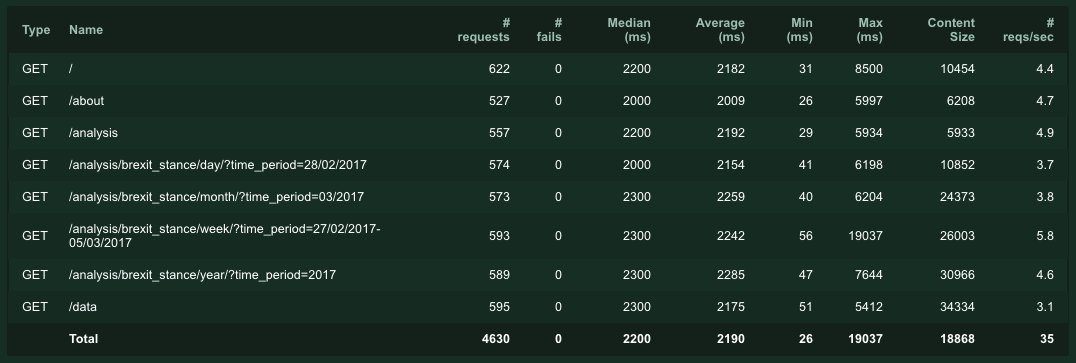
\includegraphics[width=\textwidth]{images/load-test.png}
  \captionof{figure}{Locust view of Load Testing.}
  \label{fig:locust}
\end{center}

\subsection*{Acceptance Testing}
To test against the functional and non-functional requirements identified within the Software Requirements Specification, a mix of black box and white box testing was used to comprehensively test against the set of all requirements. The result of such testing found that all requirements as identified within the system had been met. 
\\

-- See Table \ref{table:requirements} for how the System met the requirements.

-- See Table \ref{table:nonfunc-requirements} for how the System met the non-functional requirements.

\newgeometry{a4paper,left=0.75in,right=1in,top=1in,bottom=1in,nohead}
\begin{landscape}
\begin{table}[]
\centering
\label{my-label}
\begin{tabular}{ |>{\raggedright\arraybackslash}p{3.75cm}|p{1cm}|>{\raggedright\arraybackslash}p{14cm}|}
\hline
\hfil Requirement Set \hfill & REQ & Implementation  \\
\hline
\multirow{3}{*}{1. Tweet Collection} 
							   & 1.1         & The System scrapers allow for the specification of hashtags for which to collect tweets for.                                                                                           \\
							   \cline{2-3}
                                  & 1.2         & The System uses tweet selection criteria in both historic scraper and realtime scraper \\
                                 \cline{2-3}
                                  & 1.3         &  The System permanently stores the tweets it collects using the \texttt{Tweet Model} as a means of saving.\\
\hline \hline
\multirow{3}{*}{2. Tweet Tokenization} 
							   & 2.1         & The System provides a tokenization interface for manual tweet tokenization.                                                                                           \\
							   \cline{2-3}
                                  & 2.2         & The System tokenization interface accepts tweet selection criteria\\
                                 \cline{2-3}
                                  & 2.3         &  The System can tokenize a plaintext tweet into a classifiable string of tokens\\
                                  \cline{2-3}
                                  & 2.4         &  The System permanently stores the tweets it tokenizes using the \texttt{TokenizedTweet Model} as a means of saving.\\
\hline \hline
\multirow{3}{*}{3. Tweet Classification} 
							   & 3.1         & The System provides a classification interface for manual tweet classification.                                                                                           \\
							   \cline{2-3}
                                  & 3.2         & The System classification interface accepts tweet selection criteria\\
                                 \cline{2-3}
                                  & 3.3         &  The System contains a \texttt{Naive Brexit Model} and \texttt{Brexit Model} which classifies tweets on whether they are in favour (leave) or against (remain) Britain Leaving the European union \\
                                  \cline{2-3}
                                  & 3.4         &  The System contains a \texttt{Sentiment Model} wgucg classifies tweets on whether they are positive or negative towards
Britain Leaving the European union.\\
                                 \cline{2-3}
                                  & 3.5         &  The System permanently stores the tweets it tokenizes using the \texttt{TokenizedTweet Model} as a means of saving.\\
                                  \cline{2-3}
                                  & 3.6         &  The System permanently stores the tweets it classifies using the \texttt{ClassifiedTweet Model} as a means of saving.\\

\hline \hline
\multirow{3}{*}{4. Visualization} 
							   & 4.1         & The website displays all tweets the system has collected on page \texttt{data.html}.                                                                                           \\
							   \cline{2-3}
                                  & 4.2         & The System provides \texttt{analysis.html} which allows the filtering of analysis by model\\
                                 \cline{2-3}
                                  & 4.3         &  The System provides a time switcher on \texttt{classifier-analysis.html} for which analysis can be filtered by day/week/month/year\\
                                  \cline{2-3}
                                  & 4.4         &  The System displays all classifications but only a subset of top classified tweets.\\
\hline \hline
\multirow{3}{*}{5. Automation} 
							   & 5.1         & The System conducts tweet collection autonomously using the \texttt{real-time} scraper implementation.                                                                                          \\
							   \cline{2-3}
                                  & 5.2         & The System conducts tweet tokenization autonomously using asynchronous celery task \texttt{receive tweet}\\
                                 \cline{2-3}
                                  & 5.3         & The System conducts tweet classification autonomously using cron job \texttt{brexit/brexit/scripts/cron.sh} \\
                                  \cline{2-3}
                                  & 5.4         &  The System conducts tweet visualisation autonomously through dynamic \texttt{template pages}\\
\hline                                                                                                   
\end{tabular}
\caption{Requirement Implementation}
\label{table:requirements}
\end{table}
\end{landscape}
\restoregeometry % Restore the global document page margins

\begin{tabular}{ |p{2cm}||p{12.25cm}|}
 \hline
 NF-REQ & Implementation\\
 \hline
 1 & The System operates in real-time and background real-time operations occur within five minutes.\\
  \hline
 2 &   The System on average responds to HTTP requests in less than 3 seconds and has been tested with load testing.\\
  \hline
 3 & The System works across common operating systems.\\
  \hline
 4 & The System works across common browsers.\\
  \hline
 5 & The System uses JSON configuration file that allow specifying models.\\
  \hline
 6 & The System uses Django's data models which are extensible through South Migrations.\\
  \hline
 7 & The System uses supervisor to ensure it is reliably up and operating.\\
 \hline
\end{tabular}
\captionof{table}{Non-Functional Requirement Implementation}
\label{table:nonfunc-requirements}

\subsection*{Continuous Integration}
For the automated checking of the formally written unit and integration tests within the system the continuous integration environment \textit{Jenkins} was used. Jenkins as previously mentioned within \textit{Section \ref{sec:deployment}} allows for the specification of a delivery pipeline, for ensuring System correctness during deployments a test step was put into the pipeline. Upon executing the test step of the delivery pipeline, each of the tests contained in the System is run against the new System to ensure the previous behaviour of the System is upheld when new changes have been implemented. If the tests fail within the execution of the test step, Jenkins records the build as a fail, and the deployment is abandoned allowing for the problematic changes to be caught early. Continuous integration ensures the system can be tested in a clean environment (created by the build step) on the Jenkins server thus providing confidence in the functionality of the System as the Jenkins environment is reflective of that of the final destination of the remote local production server. See Figure \ref{fig:test-trend} for the Jenkins view of continuous integration testing of previous deployments through a test result trend chart.

\begin{center}
  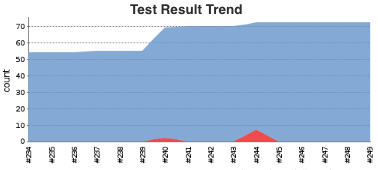
\includegraphics[width=0.6\textwidth]{images/test-trend.png}
  \captionof{figure}{Jenkins view of Continuous Integration testing of deployments.}
  \label{fig:test-trend}
\end{center}
\end{document}